\chapter{A local observable for linear lattice imperfections}
\label{ch_localobs}

\newcommand{\combtoangle}[3]{
  $\SI{#1}{\degree} - \SI{#2}{\degree} - \SI{#3}{\degree}$
}

\newcommand{\noiserms}{$0.7\times 10^{-3}\times 2\pi$ rad{}}
\newcommand{\highnoise}{$1.8\times 10^{-3}\times 2\pi$ rad{}}

\newcommand{\maxfigwidth}{8.5cm}


\section{Introduction}

Linear optics corrections have achieved remarkable performance in the last years
\cite{Tomas2017, Tomas2012, Persson2017, Aiba2013, Sagan2000, Borer1983, Langner2015},
pushing the precision and accuracy of $\beta$ function and transverse coupling
measurements further.

Special accelerator segments like the interaction regions of colliders
need a precise control of local optics which becomes a challenging task
if the optics are pushed to more extreme settings. New methods and more
precise hardware are required to measure and correct machine
imperfections such as quadrupole errors. In the case of a collider the
exact measurement and control of the $\beta$ function at the interaction point is important for operation of
the machine and to optimise luminosity~\cite{jaime}.

%For the correction of nonlinear lattice imperfections, resonance driving terms can successfully be
%used. This technique is performed successfully in the routine optics measurement and correction of
%LHC \cite{Persson2013}. \smallquest{are there others that use rdts?}

In order to locate error sources we are interested in local
observables, i.e. terms that only depend on lattice parameters and error sources in a localised
region. Such a local observable does not exist for linear lattice imperfections. For the non-linear
ones one has been found so far
\cite{Tomas2005, Franchi2007}: 
%
\begin{align}
  \chi(N) =& \frac{\hat{x}_1(N)}{\cos \left( \varphi_{x,12} - \frac{\pi}{2} \right)} 
  + \frac{\hat{x}_3(N)}{\cos\left( \varphi_{x,23}-\frac{\pi}{2} \right)} \notag \\
  &+ \hat{x}_2 (N) \left(
    \tan\left( \varphi_{x,12}-\frac{\pi}{2} \right)
    + \tan\left( \varphi_{x,23}-\frac{\pi}{2} \right)
  \right)
  \fstop
  \label{eq_chi}
\end{align}
%
$\chi (N)$ is built with the signal of three beam position monitors at positions $s_1, s_2, s_3$.

An extension of $\chi(N)$ into the linear regime does not seem possible since measured amplitude
and phase are used in a way to remove information on the linear beam dynamics.

Certain optics parameters (e.g. the $\beta$ function or coupling) can be calculated from the phase
advances between two or three BPMs \cite{Franchi2010, Miyamoto2010, Castro1996}
independently from BPM calibration errors \cite{Calaga2007}. 
The phase advance measured from a Fourier Transform \cite{Guo2016} turn-by-turn data is independent of the amplitude
of the signal and, thus, not affected by calibration errors.
%For coupling measurements, a reconstruction of the complex signal is necessary which requires using
%the amplitude \cite{Miyamoto2010}. The dependence on calibration can, in this case, be eliminated by using normalising
%the spectral lines by the main tune line.

%The $\beta$ function algorithms use only the phase advance which is independent of calibration errors
%whereas the coupling algorithm needs also the amplitude of the given spectral line. It is possible
%to remove the dependence on BPM calibration by taking the amplitude normalised to the main tune line.

The phase advance between two elements of an accelerator depends, in general, on all the elements in
the ring.
%Therefore, all lattice imperfections in the machine alter the phase advance between two
%arbitrary positions.


Under the assumption that coupling and higher order imperfections are negligible we
study the effect of quadrupolar field errors on the phase advance up to first order and construct an observable for
linear lattice imperfections that is local. For second order considerations we find a formula
for phase beating but global contributions cannot be eliminated.

The focus of this work lies on circular machines where phase advance can be measured accurately by
exciting an oscillation of the beam.
Excitation methods include single kicks and driven oscillation by an AC-dipole \cite{Miyamoto2008} which
generate a stable coherent motion of the beam.
Conceptually the local observable described in this work applies also to linear machines but accurate measurements
of phase advances remain challenging and the application of the proposed technique might not be practical.
Instead model-based fitting methods \cite{Zhang2018}
might be more suited to retrieve optics parameters directly.

%This article is organised in the following structure:
%
%Section \ref{sec:localobs} derives a local expression from the phase advance beating. This
%expression depends solely on the phase advances between four different BPMs.
%It reduces to just two BPMs if their mutual
%model phase advance is an exact multiple of $\pi$. 
%
%Section \ref{sec:robustness_check} examines the robustness of the local observable against noise and
%explores the visibility of strong error sources in the arc.
%
%Section \ref{sec:measurements} shows an example of a real LHC measurement of the local observable
%and the results are discussed.


% --------------------------------------------------------------------------------------------------
% ----- MAIN SECTION -------------------------------------------------------------------------------
% --------------------------------------------------------------------------------------------------

\section{Local observable}
\label{sec:localobs}


The effect of linear
lattice imperfections on the resonance driving terms (RDTs) and their impact on the betatron phase is
studied.
We express the betatron motion in the language of normal form and Courant-Snyder coordinates
\cite{Bartolini1997}.

The phase beating due to quadrupolar field errors is given by \eqref{eq_phasebeating_1st_app}.
$\bar{h}_{ij}$ only depends on quadrupole errors inside the range $[i,j]$ and is therefore a local
term. The RDTs $f_i$ in \eqref{eq_phasebeating_1st_app}, on the other hand, contain global contributions.

The following subsections describe the derivation of an expression for local phase beating in two distinct
cases: The first is the general case with arbitrary phase advances between the BPMs. A combination of
four BPMs is necessary to calculate a pure local term. The second case considers only two BPMs with a
phase advance of $\pi$.

\subsection{The general case -- phase advances different from \texorpdfstring{$n\pi$}{n*pi}}
\label{sec_generalcase}
%
\begin{figure}[htbp]
%\begin{wrapfigure}{O}[\figborderhang]{5cm}
  \centering
    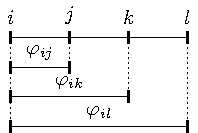
\includegraphics[width=.3\linewidth]{figIntervPhiIj}
  \caption{The interval of BPMs with corresponding phase advances.}
  \label{fig_interv_phi_ij}
%\end{wrapfigure}
\end{figure}
%
\equationref{eq_phasebeating_1st_app} still carries a dependence on the global error distribution in the form
of the terms $f_i$. We can eliminate those terms by carefully summing up phase advances between
different pairs of BPMs.


% --------------------------------------------------------------------------------------------------
\section{Eliminating global contributions}
\label{sec_resummation}
The goal of this section is to eliminate global contributions to \eqref{eq_phasebeating_1st_app}.
This can be achieved a careful resummation of phase advances between four BPMs.

The global term $\re{f_i}$ can be eliminated by taking a third BPM $k$ and divide by the respective factor:
%
\begin{equation}
	\frac{\Delta\varphi_{ij}}{\sin^2\varphi_{ij}\m} - \frac{\Delta\varphi_{ik}}{\sin ^2\varphi_{ik}\m}
  =
	\frac{
    \bar{h}_{ij}
  }{
    \sin^2\varphi_{ij}\m
  } -
  \frac{
    \bar{h}_{ik }
  }{
    \sin^2\varphi_{ik}\m
  }
  - 8\left(\cot\varphi_{ij}\m - \cot\varphi_{ik}\m\right)\im{f_i}
    \fstop
    \label{eq_Deltaphi_first_step}
\end{equation}
%
Proceeding similarly with the factor in front of $\im{f_i}$:
%
\begin{equation}
  \frac{
    \frac{\Delta\varphi_{ij}}{\sin^2\varphi_{ij}\m} - \frac{\Delta\varphi_{ik}}{\sin ^2\varphi_{ik}\m}
  }{
    \cot\varphi_{ij}\m - \cot\varphi_{ik}\m } =
  \frac{
    \frac{ \bar{h}_{ij} }{ \sin^2\varphi_{ij}\m } -
    \frac{ \bar{h}_{ik } }{ \sin^2\varphi_{ik}\m }
  }{
    \cot\varphi_{ij}\m - \cot\varphi_{ik}\m
  }
  - 8\im{f_i}
    \fstop
    \label{eq_Deltaphi_second_step}
\end{equation}
%
We can simplify the lhs to:
{
\small
%
\begin{align}
  \frac{
    \frac{\Delta\varphi_{ij}}{\sin^2\varphi_{ij}\m} - \frac{\Delta\varphi_{ik}}{\sin ^2\varphi_{ik}\m}
  }{
  \cot\varphi_{ij}\m - \cot\varphi_{ik}\m }
  =&  \frac{\Delta\varphi_{ij}}{
    \sin^2\varphi_{ij}\m \left( \cot\varphi_{ij}\m - \cot\varphi_{ik}\m \right)
  }
  -
  \frac{\Delta\varphi_{ik}}{
    \sin^2\varphi_{ik}\m \left( \cot\varphi_{ij}\m - \cot\varphi_{ik}\m \right)
  } \notag \\
  =&
  \frac{
    \Delta\varphi_{ij}\sin\varphi_{ij}\m \sin\varphi_{ik}\m
  }{
    \sin^2\varphi_{ij}\m \left( \cos\varphi_{ij}\m \sin\varphi_{ik}\m - \cos\varphi_{ik}\m\sin\varphi_{ij}\m \right)
  }\notag \\
  &-
  \frac{
    \Delta\varphi_{ik}\sin\varphi_{ij}\m \sin\varphi_{ik}\m
  }{
    \sin^2\varphi_{ik}\m \left( \cos\varphi_{ij}\m \sin\varphi_{ik}\m - \cos\varphi_{ik}\m\sin\varphi_{ij}\m \right)
  } \notag  \\
  =& 
  \frac{
    \Delta\varphi_{ij}\left( 
    \sin \varphi_{ij}\m \cos \varphi_{jk}\m + \cos \varphi_{ij}\m \sin\varphi_{jk}\m\right)
  }{
    \sin\varphi_{ij}\m \sin \varphi_{jk}\m
  } \notag \\
  &-
  \frac{
    \Delta\varphi_{ik}\left( 
    \sin \varphi_{ik}\m \cos \varphi_{jk}\m - \cos \varphi_{ik}\m \sin\varphi_{jk}\m\right)
  }{
    \sin\varphi_{ik}\m \sin \varphi_{jk}\m
  } \notag \\
  =&
  \Delta\varphi_{ij} \left( 
    \cot \varphi_{ij}\m + \cot\varphi_{jk}\m
  \right)
  -
  \Delta\varphi_{jk} \left( 
    \cot\varphi_{jk}\m - \cot\varphi_{ik}\m
  \right)
  \fstop
\end{align}
%
}
The rhs of \eqref{eq_Deltaphi_second_step} can be simplified analogously and we can rewrite it to
%
\begin{align}
  & \Delta\varphi_{ij} \left( 
    \cot \varphi_{ij}\m + \cot\varphi_{jk}\m
  \right)
  -
  \Delta\varphi_{jk} \left( 
    \cot\varphi_{jk}\m - \cot\varphi_{ik}\m
  \right) \notag \\
  =& 
  \bar{h}_{ij} \left( 
    \cot \varphi_{ij}\m + \cot\varphi_{jk}\m
  \right)
  -
  \bar{h}_{jk} \left( 
    \cot\varphi_{jk}\m - \cot\varphi_{ik}\m
  \right)
  - \im{f_i}
  \fstop
  \label{eq_simplify_second_step}
\end{align}
%
To finally eliminate $\im{f_i}$ we take a fourth BPM, $l$, and subtract 
%
\begin{equation}
   \Delta\varphi_{ij} \left( 
    \cot \varphi_{ij}\m + \cot\varphi_{jl}\m
  \right)
  -
  \Delta\varphi_{jl} \left( 
    \cot\varphi_{jl}\m - \cot\varphi_{il}\m
  \right) \notag \\
  \label{eq_fourth_bpm}
\end{equation}
%
from \eqref{eq_simplify_second_step} and end up with
%
\begin{align}
 &\cot\varphi_{jl}\m \left( \Delta\varphi_{il} - \Delta\varphi_{ij} \right) 
 + \cot\varphi_{jk}\m \left( \Delta\varphi_{ij} - \Delta\varphi_{ik} \right) 
 - \cot\varphi_{ki}\m \Delta \varphi_{ik} + \cot\varphi_{li}\m\Delta\varphi_{il}\notag  \\
 =& 
 \cot\varphi_{jl}\m \left( \bar{h}_{il} - \bar{h}_{ij} \right) 
 + \cot\varphi_{jk}\m \left( \bar{h}_{ij} - \bar{h}_{ik} \right)
 - \cot\varphi_{ki}\m \Delta \varphi_{ik} + \cot\varphi_{li}\m\bar{h}_{il} 
\fstop
\label{eq_full_lhs_rhs}
\end{align}
%
Figure~\ref{fig_thetacomb} illustrates the collection of four BPMs used to construct
\eqref{eq_full_lhs_rhs}.
The left hand side of \eqref{eq_full_lhs_rhs} can be further simplified to
%
\begin{align}
 &\cot\varphi_{jl}\m \left( \Delta\varphi_{il} - \Delta\varphi_{ij} \right) 
 + \cot\varphi_{jk}\m \left( \Delta\varphi_{ij} - \Delta\varphi_{ik} \right) 
 - \cot\varphi_{ki}\m \Delta \varphi_{ik} + \cot\varphi_{li}\m\Delta\varphi_{il} \notag\\
 =&\cot\varphi_{jl}\m \Delta\varphi_{jl} - \cot\varphi_{jk}\m \Delta\varphi_{jk}
+ \cot\varphi_{ik}\m\Delta\varphi_{ik} - \cot\varphi_{il}\m\Delta\varphi_{il}
\fstop
  \end{align}
%
  Now we can rewrite \eqref{eq_full_lhs_rhs} as
%
\begin{equation}
  \Phi_{ijkl}^{\mathrm{meas}} = \Phi_{ijkl}^{\mathrm{model}} 
  \label{eq_Deltaphi_model_meas_app}
\end{equation}
%
by defining
%
\begin{align}
  \Phi^{\mathrm{meas}}_{ijkl} \equiv&
  \cot\varphi_{jl}\m\Delta\varphi_{jl} - \cot\varphi_{jk}\m\Delta\varphi_{jk}
  + \cot\varphi_{ik}\m\Delta\varphi_{ik} - \cot\varphi_{il}\m\Delta\varphi_{il} 
  \label{eq_deltaphi_firstorder_app}
\end{align}
%
and
%
\begin{align}
  \Phi_{ijkl}^\text{model} \equiv&
  \cot\varphi_{jl}\m\left(\bar{h}_{il} - \bar{h}_{ij}\right) 
  -\cot\varphi_{jk}\m\left( \bar{h}_{ij} - \bar{h}_{ik} \right)
  + \cot\varphi_{ik}\m \bar{h}_{ik} - \cot\varphi_{il}\m\bar{h}_{il}
  \fstop
  \label{eq_analyticalphi_firstorder_app}
\end{align}
%
Those terms are truly local to the region in between the four BPMs.


The resummation yields an observable
%
\begin{align}
  \Phi^{\mathrm{meas}}_{ijkl} =&
  \cot\varphi_{jl}\m\Delta\varphi_{jl} - \cot\varphi_{jk}\m\Delta\varphi_{jk} \notag \\
  &+ \cot\varphi_{ik}\m\Delta\varphi_{ik} - \cot\varphi_{il}\m\Delta\varphi_{il} 
  \label{eq_deltaphi_firstorder}
\end{align}
%
which only depends on measured phase advances between the four BPMs $i$, $j$, $k$ and $l$.
Up to first order it is equal to an analytic expression
%
\begin{align}
  \Phi_{ijkl}^\text{model} =&
  \cot\varphi_{jl}\m\left(\bar{h}_{il} - \bar{h}_{ij}\right) 
  -\cot\varphi_{jk}\m\left( \bar{h}_{ij} - \bar{h}_{ik} \right) \notag \\
  &+ \cot\varphi_{ik}\m \bar{h}_{ik} - \cot\varphi_{il}\m\bar{h}_{il}
  \label{eq_analyticalphi_firstorder}
\end{align}
%
which depends only on local error sources.
There are no global contributions left and the two quantities defined in Eqs. (\ref{eq_deltaphi_firstorder}) and 
(\ref{eq_analyticalphi_firstorder}) are truly local up to first order.
%
\begin{figure}
%\begin{wrapfigure}{O}[\figborderhang]{5cm}
  \centering
  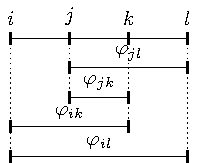
\includegraphics[width=.3\linewidth]{figThetaComb}
\caption{
  The phase advances appearing in Eqs.~(\ref{eq_deltaphi_firstorder}) and (\ref{eq_analyticalphi_firstorder}).
  The phase advances $\varphi_{ij}$ and $\varphi_{kl}$ do not appear in the final form of the local
  observable.
}
  \label{fig_thetacomb}
%\end{wrapfigure}
\end{figure}
%
The measurement uncertainty can be propagated to $\Phi_{ijkl}^\text{meas}$:
%
\begin{align}
  \sigma_\Phi^2 =& 
    \cot^2\varphi_{jl}\m \sigma_{\varphi_{jl}}^2
    + \cot^2\varphi_{jk}\m \sigma_{\varphi_{jk}}^2 \notag \\
    &+ \cot^2\varphi_{ik}\m \sigma_{\varphi_{ik}}^2 
    + \cot^2\varphi_{il}\m \sigma_{\varphi_{il}}^2
  \fstop
  \label{eq_Phi_err}
\end{align}
%
Equation~(\ref{eq_Phi_err}) is used to calculate the size of the errorbars in local observable plots.

A consideration of degrees of freedom suggests that three BPMs should suffice to reconstruct
the local linear optics errors. However, this reconstruction would depend on the amplitude which,
in turn, may suffer from calibration errors. The local observable presented here is independent of
BPM calibration errors.
%
\begin{figure}[h]
  \centering
  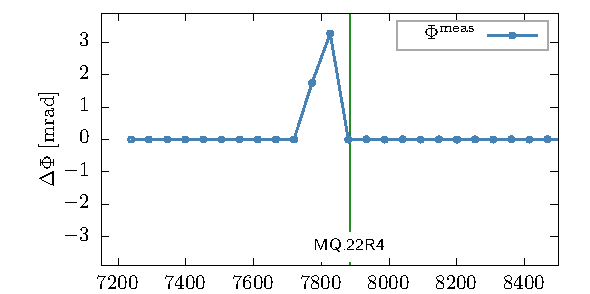
\includegraphics[width=.7\linewidth]{./sim_locality.pdf}
  \caption{The impact of a focusing error on the local observable. The plot shows an LHC arc with a
    relative error of $\SI{0.1}{\percent}$ of the magnetic field of focusing quadrupole \texttt{MQ.22R4}
    which is marked by a vertical line.
  }
  \label{fig_locality}
\end{figure}
%
Figure~\ref{fig_locality} illustrates the impact of a quadrupole error on the local observable.
The plot shows an LHC arc with $\SI{90}{\degree}$ FODO cells. Two BPMs are placed in one FODO cell, directly
in front of the focusing or defocusing quadrupoles, respectively.
The BPMS $i$, $j$, $k$ and $l$ are chosen to be consecutive ones.
A relative field error of $\SI{0.1}{\percent}$ was introduced at magnet \texttt{MQ.22R4}. Since the
points corresponding to a value of $\Phi_{ijkl}^\text{meas}$ are placed at the position $s_i$, only
the three points that precede the introduced error are affected, for which the introduced error lies
in the interval $[s_i, s_l]$.
The first of the three affected points has a very small value because of the proximity of the quadrupole
to the BPM.

\subsection{Exact multiples of \texorpdfstring{$\pi$}{pi}}

If the model phase advance is $\varphi_{ij}\m = n\pi$, the phase advance beating between two positions,
\eqref{eq_phasebeating_1st_app} reduces to
%
\begin{equation}
 % \phi_{ij}^\text{model} \equiv
  \Delta\varphi_{ij} = \bar{h}_{ij}
  \komma
  \label{eq_npi_localobs}
\end{equation}
%
which implies that $\Delta \varphi_{ij}$ is directly a local observable when
$\varphi_{ij}^\text{m}=n\pi$.
In this case the number of BPMs is reduced to two at positions $i$ and
$j$.
In general, phase advances that are sufficiently close to multiples of $\pi$ might not be present in
standard operation of an accelerator -- an exception is for example the ATS optics
\cite{Fartoukh2013} that is now used
in LHC and which is the proposed baseline for its high luminosity upgrade --, but it would be conceivable to prepare
special optics settings for a corresponding measurement in any acclerator.
The error of the local observable in this case,
%
\begin{equation}
    \sigma_{\Delta\varphi_{ij}} = \sigma_{\varphi_{ij}}
    \komma
    \label{eq_error_npi}
\end{equation}
%
is smaller than for the general local observable.

\subsection{Exploring the second order}
\label{ssec:second_order_phasebeating}

The details of the second order calculations can be found in the appendix. Here we summarise the results.
The detuning hamiltonian term $h_{1100,ij} $ as well as the RDT $f_{i} $ have to be extended to second order:
%
\begin{align}
  h_{1100,ij} &\rightarrow h_{1100,ij}^{(1)} + h_{1100,ij}^{(2)}\\
  f_{i} &\rightarrow f_{i}^{(1)} + f_{i}^{(2)}
  \fstop
  \label{eq_1st--2nd}
\end{align}
%
The total phase advance beating is, then,
%
\begin{align}
  \Delta\varphi_{ij} = &-2h_{1100,ij}^{(1)} 
  - 2h^{(2)}_{1100,ij}
  + 4\re{f_j^{(1)} - f_i^{(1)}} \notag\\
  &+ 4\re{f_j^{(2)} - f_i^{(2)}}\notag \\
  &+ 16 \left( \re{f_j^{(1)}} \im{f_j^{(1)}} - \re{f_i^{(1)}} \im{f_i^{(1)}} \right)\notag\\
  &+ O(K^{3})
  \fstop
  \label{eq_phadvbeating_2nd_inline}
\end{align}
%
The same resummation techniques as for the first order will not suffice to eliminate
global RDTs $f_i$ and $f_j$.
If we reformulate the third line of \eqref{eq_phadvbeating_2nd_inline} as
%
\begin{align}
   \re{f_j} \im{f_j} - \re{f_i} \im{f_i}  = 
   \frac{1}{2}\im{f_j^2} - \frac{1}{2}\im{f_i^2} \notag \\
    = \frac{1}{2} \im{ 
     A_{ij}^2 + 2A_{ij}f_i\e{2i\varphi_{ij}\m} + 
     \left( \e{4i\varphi_{ij}\m} - 1 \right) f_{i}^2}
  \label{eq_expanding2ndorder}
\end{align}
%
we see that it is not possible to separate the global $f_i$ from the local term $A_{ij}$. This
separation was the key to be able to eliminate the global terms in the first order approximation.

For $\varphi_{ij}\m = n\pi$ a second order term can be derived analogously:
%
\begin{align}
  \Delta\varphi_{ij} = & \bar{h}_{ij} - 2h_{1100,ij}^{(2)} \notag \\
  &+ 4\re{f_j^{(2)}-f_i^{(2)}} + 8\im{A_{ij}^{2}+ 2A_{ij}f_i}
  \fstop
  \label{eq_npi_second}
\end{align}
%
This term also contains the global $f_1$ and $f_2$ and there are no common factors that can be exploited
to eliminate them.

Therefore in this work purely local observable cannot be extracted from the second order phase beating.

% --------------------------------------------------------------------------------------------------
% ----- lobster ------------------------------------------------------------------------------------
% --------------------------------------------------------------------------------------------------

\section{Simulating Errors and Noise}
\label{sec_lobster}
\label{sec:robustness_check}

\subsection{General simulation setup}

In order to assess the usability of the local observable we perform a series of simulations with different
quadrupole error distributions and compare the prediction of the analytical calculations with simulated results. 
We base our simulations on the nominal LHC lattice at the end of run~II in 2018 with ATS optics and 
$\beta^*=\SI{30}{\centi\metre}$.

Figure~\ref{fig_combination} shows a sketch of a typical LHC arc section. BPMs are placed directly in
front of the quadrupoles of FODO cells. Additional trim quadrupoles (e.g. MQT) may be present.
%
\begin{figure}[htbp]
%\begin{wrapfigure}{O}[\figborderhang]{6cm}
  \centering
  \includestandalone[width=.5\linewidth]{figcombination}
  \caption{The probed interval $I_p$ for a typical section inside an LHC arc.
    BPMs are represented by rectangles.
    The phase advance between to consecutive BPMs is approximately $\SI{45}{^\circ}$.
    Used BPMs are shown in orange, unused in gray.
    Blue diamonds indicate quadrupoles and trim quadrupoles.
    Only BPMs and quadrupoles are shown, other elements such as corrector spool pieces and the
    bending dipoles are omitted.
  }
  \label{fig_combination}
\end{figure}
%
%\end{figure}
%
Four cases will be studied: the first one is a set of LHC design field
errors from WISE~\cite{wise1,wise2}, shown in Tab.~\ref{tab_design}, in the absence of phase noise.
This setup will let us verify the equality of Eqs.~(\ref{eq_deltaphi_firstorder}) and (\ref{eq_analyticalphi_firstorder}).
Then Gaussian noise of \noiserms{} is added to the simulated phase advances to illustrate the behaviour
in the presence of noise.
A third simulation includes an additional strong error source in one of the quadrupoles, c.f. Tab.~\ref{tab_design_peak}
to demonstrate the impact of single strong error sources and the locality of the local observable.
A last simulation setup demonstrates the visibility of quadrupolar errors originating from feed-down
of sextupoles via orbit offsets.

\begin{table}
  \begin{center}
    \begin{tabular*}{.5\textwidth}{l @ {\extracolsep{\fill}} c}
      Element & $\sigma_{K_1}/K\; [10^{-4}]$ \\
      MQ  & 12\\
      MQT & 75\\
      MQM & 12\\
      MQY & 11\\
      MQW & 15\\
      MQX & 1\\
      MB & 4\\
    \end{tabular*} \\
    \caption{Error distribution for the design LHC lattice at $\SI{6.5}{TeV}$ with weak errors in the final triplet in
      order to avoid higher order effects.
      $K$ denotes the main field component (quadrupolar field for quadrupoles, etc).
    }
   \label{tab_design}
  \end{center}
\end{table}

\begin{table}
  \begin{center}
    \begin{tabular*}{.5\textwidth}{l @ {\extracolsep{\fill}} c c}
      Element & $\delta K_1/K\; [10^{-4}]$ & $\sigma_{K_1}/K\; [10^{-4}]$ \\
      MQ.22R4.B1 & 100 & -\\
      MQ  & - & 12\\
      MQT & - & 75\\
      MQM & - & 12\\
      MQY & - & 11\\
      MQW & - & 15\\
      MQX & - & 1\\
      MB &-& 4 \\
    \end{tabular*}
    \caption{
      In addition to design LHC errors distribution we introduced a single strong error source in
      arc45.
    }
    \label{tab_design_peak}
  \end{center}
\end{table}

There are many different possible combinations of BPMs. In the following comparison plots we will only show
two of them: one that has a phase advance of $\SI{180}{\degree}$ in one of the phase advances appearing in
Fig.~\ref{fig_thetacomb_ij-kl} and one that avoids such a term and,
additionally, the 2-BPM combination with $\varphi_{ij}=\SI{180}{\degree}$.

In a real measurement we would consider only the combinations of closest BPMs to avoid the
accumulation of systematic errors coming from other lattice elements and therefore we limit our study
to only those combinations.
The phase advance over two FODO cells in telescopic arcs of the ATS optics is tightly matched
to $\pi$. On the one hand this provides a continuous set of combinations with
similar phase advances and thus we can more easily compare the values of $\Phi_{ijkl}^\text{model}$
and $\Phi_{ijkl}^\text{meas}$ at different positions.
On the other hand this gives rise to model phase advances close to multiples of $\pi$ for several
combinations which gives the possibility to explore these cases.
Table~\ref{tab_combs} shows the closest combinations with all occuring model phase advances.
Reflected combinations are omitted. Model phase advances close to $n\pi $ cause the cotangent
terms to diverge. They are therefore highlighted in red.
Since we still want to study these cases and avoid divergences and the resulting numerical instabilies
we impose a filter on the phase advances. 
Those which are closer to $n\pi$ than $10^{-6}\times 2\pi$ are excluded. 
The case \combtoangle{45}{90}{45} is sketched in Fig.~\ref{fig_thetacomb_ij-kl}.
%
\begin{figure}
  \centering
  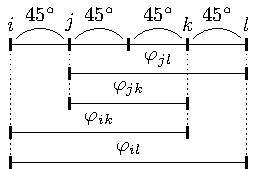
\includegraphics[width=.3\linewidth]{figThetacombijkl}
  \caption{The phase advances of the combination
    $\varphi_{ij}=\SI{45}{\degree}$, $\varphi_{jk}=\SI{90}{\degree}$, $ \varphi_{kl}=\SI{45}{\degree}$.
The phase advance $\varphi_{il} = \SI{180}{\degree}$ causes $\cot\varphi_{jl}\m$ to diverge.
  }
  \label{fig_thetacomb_ij-kl}
\end{figure}
%
%$cot n\pi = \infty$ for $n \in \mathbb{Z} $, so 

\begin{table}[htbp]
    \begin{center}
    % #publish_picture figTable1
    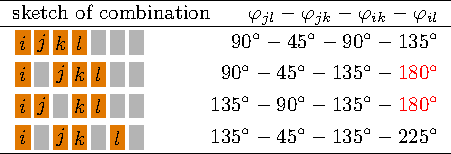
\includegraphics{figTable1}
    \end{center}
    % #end publish_picture
    \caption{Indices $i,j,k,l$ and phases appearing model phase advances for the closest combinations.
      The actual model phase advances depend on the respective model settings and differ slightly from
      the exact values above.
    }
    \label{tab_combs}
\end{table}

Model and measurement values are shown for the combinations \combtoangle{45}{45}{45} and
\combtoangle{90}{45}{45} and $\varphi_{ij}\m = \SI{180}{^\circ}$ in Figures~\ref{fig_design_nonoise}~to~\ref{fig_peak_noise}.
Since we get the phase advances of Table~\ref{tab_combs} only for telescopic arcs and for the sake
of readability we limit the plot region to just one telescopic arc, the one between IR4 and IR5.
For simplicity we show only results for the horizontal plane. 


\subsection{Design field errors}

The first case, Fig.~\ref{fig_design_nonoise}, is free of noise with the quad error distribution of
Tab.~\ref{tab_design}.
The agreement between analytical and measurement values is excellent, showing the validity of
Eqs.~(\ref{eq_deltaphi_firstorder}), (\ref{eq_analyticalphi_firstorder}) and (\ref{eq_npi_localobs}).

\newcommand{\errdist}{design}
%
\begin{figure}
  \centering
  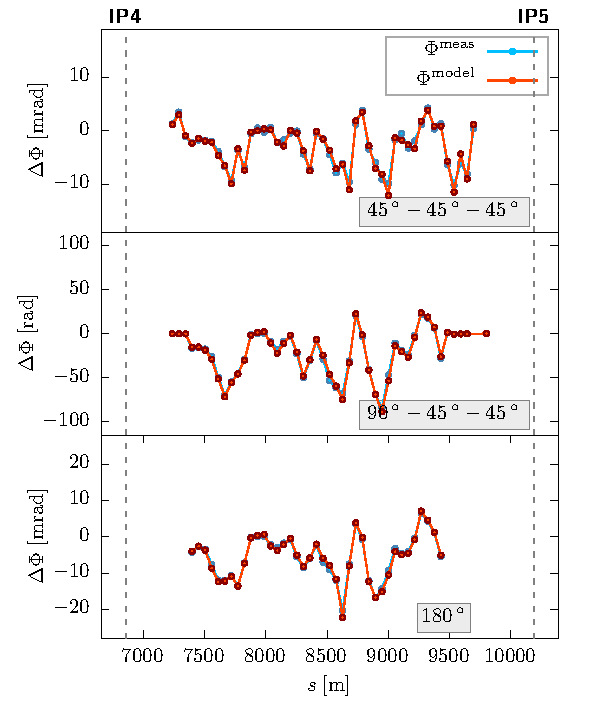
\includegraphics[width=.8\linewidth]{sim_no_noise}
  %\includegraphics[width=\linewidth]{./73_plots/sim_ij-kl_design_IP4}
  \caption{
    This figure shows the first two combinations of Tab.~\ref{tab_combs} and the case $\varphi_{ij}\m = \pi$
    from simulations.
    Top: the combination \combtoangle{45}{45}{45}.
    Center: the combination $\SI{90}{\degree}-\SI{45}{\degree}-\SI{45}{\degree}$. The absolute value of the local observable in the telescopic arc
    (right of IP4) is four orders of magnitude higher than in the top plot.
    The plots only show values where the phase advances do not differ more than $\SI{1}{\degree}$
    from the target values displayed in Tab.~\ref{tab_combs} in order to ensure comparability between
    the values. Additionally values with a model phase advance in $n\pi \pm 10^{-6}$ are excluded
    to avoid numerical instabilities.
    This causes the IR to be empty of local phase advances. 
    Note that in the middle plot the values are four orders of magnitude higher than in the other two.
    This originates from the $\cot\varphi_{il}\m$ terms which are high because of $\varphi_{il}\m \approx \pi$.%Values in non-telescopic arcs are strongly suppressed.
    The bottom plot shows the local observable for model phase advances of $\SI{180}{^\circ}$. 
    In all three plots the agreement between model and simulation is excellent.
  }
  \label{fig_design_nonoise}
\end{figure}
%
To examine the behaviour of the local observable in the vicinity of $n\pi$ we have to scan the accelerator
for available model phase advances. For each BPM $i$ we are looking for a second one -- BPM $j$ -- that
is placed at $\Delta\varphi_{ij} = \pi\pm\delta\phi$ downstream.
$\delta\phi$ is a threshold parameter controlling how many local observable pairs are accepted.
We chose $\delta\phi=\SI{1e-3}{}\times2\pi$.
The telescopic arcs of the ATS optics provide the needed model phase advances.

The agreement is, as for the general case, very good in the absence of errors.

\subsection{Phase noise}

The noise to signal ratio decreases with increasing oscillation amplitude and thus with increasing
$\beta$ function at the BPM. In the LHC FODO cells BPMs are installed close to the focusing and
defocusing quadrupoles and those lie at $\beta$ function maxima and minima, respectively.
Therefore we can divide the arc BPMs in two categories, those with low $\beta$ function and those with
high $\beta$ function. The $\beta$ function minima are usually around $\SI{30}{\meter}$ and the
maxima at $\SI{180}{\meter}$.
The phase advance uncertainties $\sigma_{\varphi_{ij}}$ fall into three categories:
both BPMs have high $\beta$ function, only one of them has high $\beta$ and both have low $\beta$.

For this set of simulations we introduce phase noise which
corresponds to noise values of the LHC signal that we typically achieve taking five data acquisitions
and after cleaning \cite{Calaga2004} and harmonic analysis.
We group BPMs into the before mentionned categories and apply a Gaussian error distribution
to the phase values according to measurement statistics.

With the introduced phase noise the agreement decreases significantly (cf. Fig.~\ref{fig_design_noise}). The noise is of the same order of magnitude
as $\Phi_{ijkl}^\text{meas}$ itself.
Therefore the LHC arc quadrupolar errors cannot be identified with this phase advance resolution.
The combination \combtoangle{45}{45}{45} shows the worst behaviour under noise because the $\beta$
function alternates between high and low values from BPM to BPM and so within the four neighbouring
BPMs there are always two with low $\beta$ function.
%
\begin{figure}
  \centering
  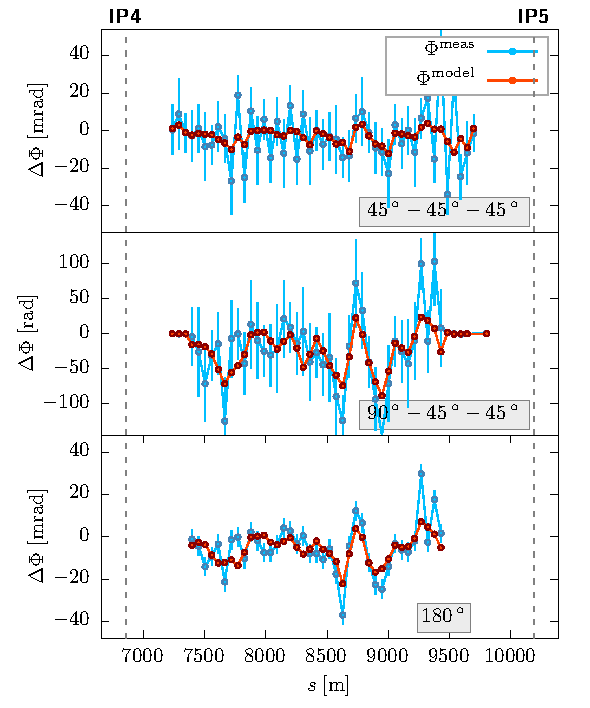
\includegraphics[width=.8\linewidth]{sim_noise} %\includegraphics[width=\linewidth]{./73_plots/sim_ij-kl_design_IP4_noise}
  \caption{
    Similar plots as in Fig.~\ref{fig_design_nonoise} but including a phase error of \noiserms{} for
    high $\beta$ function values and \highnoise{} for low $\beta$s.
    The agreement between model and simulation and measurement is highly deteriorated.
    The error bars have been calculated using Eqs. (\ref{eq_Phi_err}) and (\ref{eq_error_npi}).
    The case $\varphi_{ij}\m=\pi$ is affected less by the error since only one phase advance error
    is propagated.
  }
  \label{fig_design_noise}
\end{figure}
%
The case of exact $\pi$ phase advances shows the smallest errors as only one phase advance
error enters in the error propagation.

\subsection{Single strong error source}

For the next simulation, we assume that there is a single strong error in one of the quadrupoles. We
assign $1\%$ of relative error to MQ.22R4 to show the effect of a strong error source. Figure~\ref{fig_peak_noise}
shows that this error creates a visible peak in the local observable.
The peak in the local observable is situated immidiately in front of the location of the error source
because the plot shows the local observable at the position of BPM $i$ but the errors of the interval
$(s_i, s_l)$ enter in the calculation of the observable.

In the presence of model phase advances close to $n\pi$ the values of the local observable in the
telescopic arcs are clearly enhanced (c.f. bottom plot of Fig.~\ref{fig_design_nonoise} and
Fig.~\ref{fig_design_noise}).

The simulations above show that strong quadrupolar error sources ($\geq 1\%$) can be detected with the local
observables under the studied phase resolution.
For the detection of smaller errors a higher precision of the phase measurement would be needed.
More precise BPMs like DOROS-BPMs \cite{Gasior2011} currently installed in the LHC interaction region and a higher excitation
amplitude as well as the acquisition of a higher number of turns
can increase the resolution of the phase measurement. 
%
\begin{figure}
  \centering
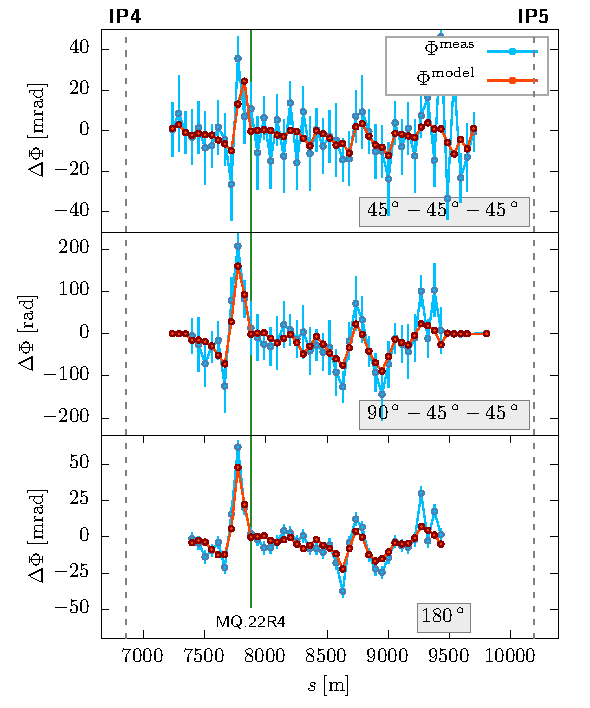
\includegraphics[width=.8\linewidth]{sim_peak}
\caption{The local observable with the error distribution of Tab.~\ref{tab_design_peak}, including
    a strong error source at \texttt{MQ.22R4.B1} and phase
    noise of \noiserms.
    %The combination \combtoangle{90}{45}{45} is less affected by the phase noise.
    The position of the strong error source is marked by a green line.
  }
  \label{fig_peak_noise}
\end{figure}
%
\subsection{Feed-down from sextupoles}

As final test case we introduce orbit offset into the machine around the IPs by activating dedicated dispersion
bumps. These are used in the ATS optics to compensate dispersion created by the crossing angles at the IPs.
The transverse displacement of the beam creates quadrupolar-like errors inside sextupoles via feed-down:
%
\begin{equation}
  \Delta K_{1,\text{sext}} = \delta x K_2
  \label{eq_sext_fedddown}
\end{equation}
%
where $\delta x$ denotes horizontal offset and $K_2$ is the strength of the sextupole. $K_{1,\text{sext}}$
can now be used for the calculation of the local observable.



Figure~\ref{fig_disp_noise} shows the local observable in this case. Regular bumps created by the
feed-down appear which are consistent in all three cases but less pronounced in the nearest neighbors case.
With the given noise level those bumps can be measured.
The local observable is not affected by feed-down in the center of the arc because sextupoles at places
with high orbit offset are turned off.
In comparison to the previous examples, Figs.~\ref{fig_design_noise} and \ref{fig_peak_noise}, the
values of the local observable did not change in this region.

The bottom plot of Fig.~\ref{fig_disp_noise} shows the changed orbit for reference.
The peaks of the local observable can be identified with the peaks in the orbit.
Again the local observable is in 
advance of the error source.
%
\begin{figure}[t]
  \centering
  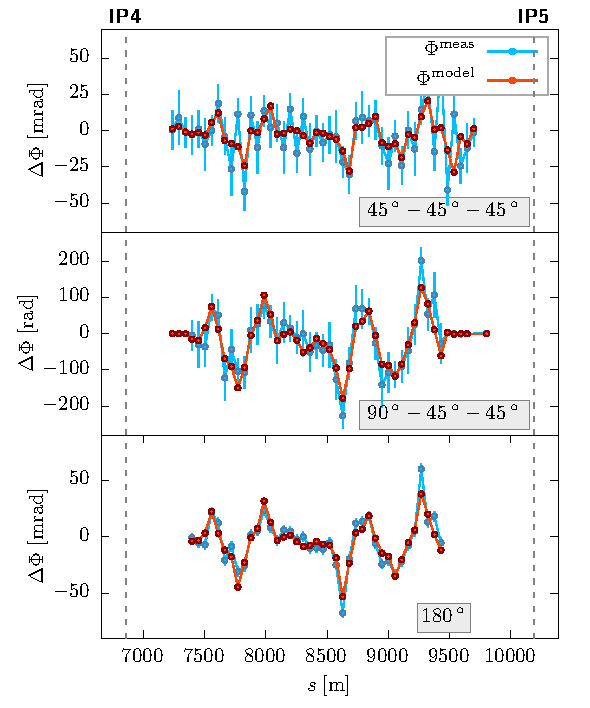
\includegraphics[width=.8\linewidth]{sim_disp}\\
  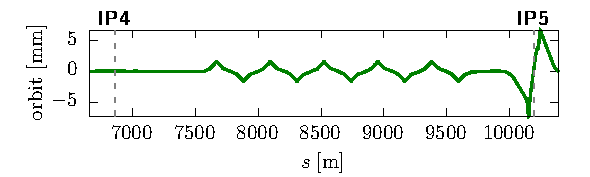
\includegraphics[width=.8\linewidth]{sim_orbit_x_noise_disp}
  \caption{The local observable with the error distribution of Tab.~\ref{tab_design} and phase noise
    of \noiserms. Additionally the orbit has been changed by dispersion bumps. The orbit offset creates
  feed-down from sextupoles.}
  \label{fig_disp_noise}
\end{figure}
%
\section{Experimental verification}
\label{sec:measurements}

\begin{figure}[t]
  \centering
  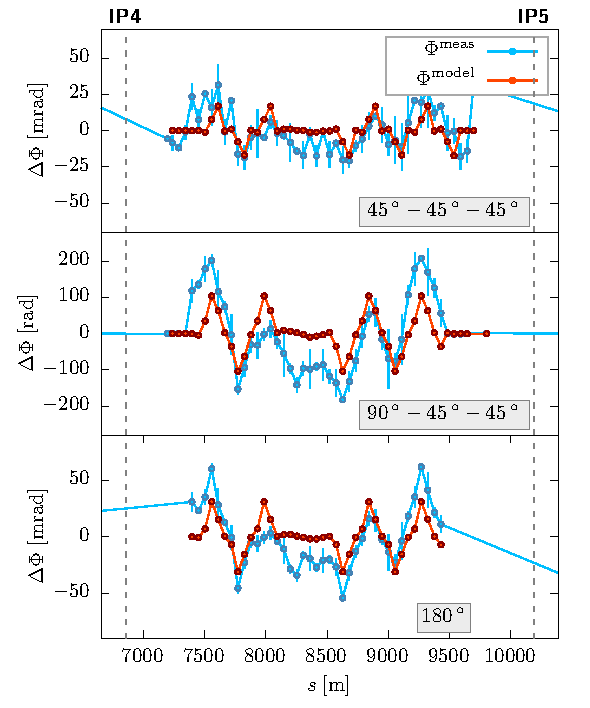
\includegraphics[width=.8\linewidth]{meas}
  %\includegraphics[width=\linewidth]{best_design_errors_meas_--l__ij-kl---}
  \caption{Plot of measurement data of the LHC commissionning 2018 at $\beta^*=\SI{30}{\centi\metre}$.
    The errorbars include statistical errors
    obtained from the phase measurement of the FFT.
    The effect of dispersion bumps on the local observable is clearly visible and matches well the
    prediction. The center region shows only a small effect from sextupoles.
  }
  \label{fig_measlobster002}
\end{figure}
%
We calculate the local observable from a measurement taken during the LHC beam commissionning in 2018.

The measurement can be seen in Fig.~\ref{fig_measlobster002} for the combinations \combtoangle{45}{45}{45}
(top plot) and \combtoangle{90}{45}{45} (bottom plot).

We take a model lattice where dispersion bumps are turned off in order to see the impact on the 
local observable.
As discussed in section~\ref{sec_lobster}, the feed-down of sextupole fields due to the orbit offset
of those bumps changes the local observable.
Figure~\ref{fig_measlobster002} shows in blue the measured local observable which features similar
spikes as the simulation (cf. Fig.~\ref{fig_disp_noise}).
In red the effect of feed-down from sextupoles via the orbit offset on the local observable is shown.
The feed down has been calculated by introducing the dispersion bump knob into the model that was turned
on during the measurement and calculating $\delta K_{1, \text{sext}}$ from \eqref{eq_sext_fedddown}.
The pattern of the model
values is also present in the measurement which confirms that their origin is indeed the feed-down.
Since the $\Phi_{ijkl}^\text{model}$ contains only the expected feed-down from sextupoles and no other
error sources (like normal quadrupole imperfections) the difference between model and measurement is
then the actual local observable created by those error sources.
The center region of the arc is free of a high peak because, as in the simulation, no sextupole is 
active at high orbit offsets.

\section{Conclusion and Outlook}

We showed the existence of a local observable for linear lattice imperfections in circular
accelerators. The locality of the observable holds up to first order in the quadrupole error
$\delta K_1$. 

Phase measurement noise is an issue with the current precision of turn-by-turn measurements and a
higher resolution in the measurement would be of advantage. For certain use cases, new techniques are
needed to improve the control of the machine and hardware upgrades are a justified solution.
Simulations show that strong error sources can be identified even with current precision of LHC measurements
as they generate distinguishable peaks.

The calculated local observable of an actual measurement shows a picture that is compatible with simulations.
Feed-down of orbit offsets via sextupoles can be seen in measurement data and be reproduced in simulations.

A future application of the observable to find strong local sources and to guide local error corrections
is foreseen for run~III of the LHC.
